\documentclass[xcolor=table]{beamer}
%------------------------------------------------------------
% Theme and Appearance
%------------------------------------------------------------
\usetheme[footline=authorinstitutetitle]{Berlin} 
\setbeamertemplate{navigation symbols}{} 

% Headline with Access Code
\setbeamertemplate{headline}{
    \begin{beamercolorbox}[wd=\paperwidth,ht=2.5ex,dp=1ex,right]{section in head/foot}
        \usebeamerfont{section in head/foot}
        \hspace{0.5cm}
        \ifnum\insertframenumber<35
            \raisebox{-1pt}[0pt][0pt]{\normalsize\textbf{Attendance Code: 542643}}
        \fi
        \hspace{0.5cm}
    \end{beamercolorbox}
}
% Footline with page numbers
\setbeamertemplate{footline}{
    \leavevmode%
    \hbox{%
        \begin{beamercolorbox}[wd=.333333\paperwidth,ht=2.25ex,dp=1ex,left]{author in head/foot}%
            \usebeamerfont{author in head/foot}\hspace*{0.5em}\insertshortauthor
        \end{beamercolorbox}%
        \begin{beamercolorbox}[wd=.333333\paperwidth,ht=2.25ex,dp=1ex,center]{title in head/foot}%
            \usebeamerfont{title in head/foot}\insertshorttitle
        \end{beamercolorbox}%
        \begin{beamercolorbox}[wd=.333333\paperwidth,ht=2.25ex,dp=1ex,right]{date in head/foot}%
            \usebeamerfont{date in head/foot}\insertshortdate{}\hspace*{2em}
            \insertframenumber{} / \inserttotalframenumber\hspace*{2ex} 
        \end{beamercolorbox}}%
    \vskip0pt%
}
\usepackage[utf8]{inputenc}
\usepackage[table]{xcolor}
\usepackage{colortbl}
\usepackage{minted}
\usepackage{lmodern}
\usepackage{tgheros}
\usepackage{hyperref}
\usepackage{tikz}
\usetikzlibrary{shapes, arrows, arrows.meta, positioning, shadows, fit, calc, backgrounds, decorations.pathreplacing}

\renewcommand*\familydefault{\sfdefault}

% Agenda at the start of every section
\AtBeginSection[]
{
    \begin{frame}
        \frametitle{Agenda}
        \tableofcontents[currentsection]
    \end{frame}
}

%------------------------------------------------------------
% Title Page Information
%------------------------------------------------------------
\title[CMP9134 - Week 13]{Release Management \& Continuous Deployment}
\subtitle{CMP9134: Software Engineering}
\author[Francesco Del Duchetto]{Dr Francesco Del Duchetto\\Lecturer in Robotics and Autonomous Systems}
\institute[University of Lincoln]{University of Lincoln}
\date{01 May 2026}

%------------------------------------------------------------
\begin{document}

%--- TITLE FRAME ---
\begin{frame}
    \titlepage
\end{frame}

%--- AGENDA FRAME ---
\begin{frame}
    \frametitle{Today's Agenda}
    \tableofcontents
\end{frame}

%------------------------------------------------------------
\section{Introduction}
%------------------------------------------------------------

\begin{frame}
    \frametitle{The Journey So Far}
    We are nearing the end of our Software Engineering journey:
    
    \begin{itemize}
        \item \textbf{Weeks 1-6:} Planning, Architecture, and Design.
        \item \textbf{Weeks 7-9:} Containerisation and Automated CI Pipelines.
        \item \textbf{Week 12:} Refactoring and Technical Debt.
    \end{itemize}
    
    \vspace{0.3cm}
    Your code is clean, containerised, and tested. The CI pipeline is green. Now comes the most terrifying part of software engineering: \textbf{Putting it in front of actual users.}
\end{frame}

\begin{frame}
    \frametitle{Deployment's Problems}
    Why is deployment historically so stressful?
    \small
    \vspace{0.1cm}
    \begin{itemize}
        \item \textbf{Downtime:} To swap in new code, you often have to shut the server down first --- meaning real users see an error page during the update (a ``Maintenance Window'').
        \item \textbf{The Unknown:} You test in a ``Staging'' environment that \textit{should} mirror live, but small differences (OS version, config, data volume) mean bugs only appear in Production --- in front of real users.
        \item \textbf{The Rollback Nightmare:} If the new version corrupts the database (e.g.\ renames a column), you cannot simply restart the old version --- it now reads data in a format it does not understand.
    \end{itemize}
    
    \vspace{0.1cm}
    \begin{block}{The Goal of Release Management}
        To make software deployments boring, routine, and virtually invisible to the end-user.
    \end{block}
\end{frame}

\begin{frame}
    \frametitle{Today's Learning Objectives}
    By the end of this lecture, you should be able to:
    \begin{enumerate}
        \item \textbf{Apply} Semantic Versioning (SemVer) to track software releases.
        \item \textbf{Differentiate} between Continuous Delivery and Continuous Deployment (CD).
        \item \textbf{Evaluate} deployment mechanics (Blue/Green, Canary Releases).
        \item \textbf{Control} feature exposure using Feature Flags (release control).
    \end{enumerate}
\end{frame}

%------------------------------------------------------------
\section{Versioning \& Tagging}
%------------------------------------------------------------

\begin{frame}
    \frametitle{What is a Release?}
    A \textbf{Release} is a specific, immutable snapshot of your software that is packaged and distributed to users or servers.
    
    \vspace{0.3cm}
    If you just push code to the `main' branch continuously, how do you know \textit{exactly} which version of the code caused the production server to crash at 3:00 AM?
    
    \vspace{0.3cm}
    We solve this through \textbf{Versioning} and \textbf{Tags}.
\end{frame}

\begin{frame}
    \frametitle{Semantic Versioning (SemVer)}
    The industry standard for versioning software is \textbf{SemVer}. It uses three numbers separated by dots: \textbf{MAJOR.MINOR.PATCH} (e.g., \texttt{v2.4.1}).
    
    \vspace{0.3cm}
    \begin{itemize}
        \item \textbf{MAJOR (\textcolor{red}{X}.y.z):} You make incompatible API changes. (If you update this, clients using the old API \textit{will} break).
        \item \textbf{MINOR (x.\textcolor{orange}{Y}.z):} You add functionality in a backwards-compatible manner. (Old clients can still use the system).
        \item \textbf{PATCH (x.y.\textcolor{green}{Z}):} You make backwards-compatible bug fixes.
    \end{itemize}

    \vspace{0.2cm}
    \textit{Note: \texttt{v0.x.x} is reserved for initial development (anything can break at any time).}
\end{frame}

\begin{frame}
    \frametitle{Think-Pair-Share: Semantic Versioning}
    \textbf{Scenario:} Your current API version is \texttt{v1.4.2}. 
    
    \vspace{0.2cm}
    Discuss with your neighbor what the \textit{new} version number should be in each of the following three independent scenarios:
    
    \begin{enumerate}
        \item You refactor a database query to make it 10x faster. The API inputs/outputs do not change.
        \item You completely delete the \texttt{/api/legacy\_stats} endpoint because nobody uses it anymore.
        \item You add an optional \texttt{?format=json} parameter to the \texttt{/api/move} endpoint.
    \end{enumerate}
    
    \pause
    \vspace{0.2cm}
    \begin{alertblock}{Answers}
        1) \textbf{v1.4.3} (Patch: Bug fix/Optimization)\\
        2) \textbf{v2.0.0} (Major: Breaking change! Clients using that endpoint will crash)\\
        3) \textbf{v1.5.0} (Minor: New feature, but old clients are unaffected)
    \end{alertblock}
\end{frame}

\begin{frame}[fragile]
    \frametitle{Git Tagging}
    Once you decide on a SemVer number, a common release workflow is to attach it to a specific Git commit. This is called a \textbf{Git Tag}.
    
    \begin{minted}[bgcolor=lightgray, fontsize=\small]{bash}
# 1. Ensure you are on the main branch
git checkout main

# 2. Create an annotated tag with a message
git tag -a v1.5.0 -m "Added optional JSON formatting"

# 3. Push the tag to GitHub
git push origin v1.5.0
    \end{minted}

    \vspace{0.2cm}
    \textbf{Why?} A Git commit hash (\texttt{a8f9c2e}) is meaningless to a human. A tag (\texttt{v1.5.0}) creates a permanent, readable bookmark in your history.
\end{frame}

%------------------------------------------------------------
\section{Continuous Deployment (CD)}
%------------------------------------------------------------

\begin{frame}
    \frametitle{Continuous Delivery vs. Continuous Deployment}
    We often hear ``CI/CD'', but the ``CD'' can mean two different things.
    
    \vspace{0.2cm}
    \begin{block}{Continuous Delivery}
        The pipeline builds, tests, and packages the code into a releasable artifact (e.g., a Docker Image). It places it in a registry. \textbf{Deployment to live servers often includes a manual approval step, depending on team policy and risk tolerance.}
    \end{block}
    
    \vspace{0.2cm}
    \begin{block}{Continuous Deployment}
        Every change that passes all stages of your production pipeline is released to your customers \textbf{automatically, with no human intervention}.
    \end{block}
\end{frame}

\begin{frame}
    \frametitle{The CD Pipeline Architecture}
    \centering
    \resizebox{0.95\textwidth}{!}{
    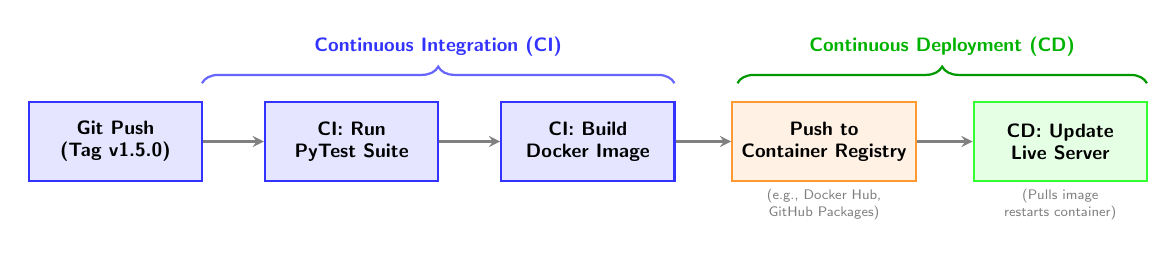
\begin{tikzpicture}[
        node distance=0.5cm and 0.5cm,
        box/.style={rectangle, draw=blue!80, fill=blue!10, thick, minimum width=2.2cm, minimum height=1cm, align=center, font=\scriptsize\bfseries},
        arrow/.style={->, >=stealth, thick, gray}
    ]
        % Nodes
        \node[box] (code) at (0,0) {Git Push\\(Tag v1.5.0)};
        \node[box] (test) at (3,0) {CI: Run\\PyTest Suite};
        \node[box] (build) at (6,0) {CI: Build\\Docker Image};
        \node[box, fill=orange!10, draw=orange!80] (registry) at (9,0) {Push to\\Container Registry};
        \node[box, fill=green!10, draw=green!80] (deploy) at (12,0) {CD: Update\\Live Server};
        
        % Arrows
        \draw[arrow] (code) -- (test);
        \draw[arrow] (test) -- (build);
        \draw[arrow] (build) -- (registry);
        \draw[arrow] (registry) -- (deploy);
        
        % Subtext
        \node[font=\tiny, align=center, text=gray] at (9, -0.8) {(e.g., Docker Hub,\\ GitHub Packages)};
        \node[font=\tiny, align=center, text=gray] at (12, -0.8) {(Pulls image\\restarts container)};

        % CI / CD brace labels
        \draw[decorate, decoration={brace, amplitude=6pt, raise=4pt}, thick, blue!60]
            (1.1, 0.6) -- (7.1, 0.6) node[midway, above=10pt, font=\scriptsize\bfseries, text=blue!80] {Continuous Integration (CI)};
        \draw[decorate, decoration={brace, amplitude=6pt, raise=4pt}, thick, green!60!black]
            (7.9, 0.6) -- (13.1, 0.6) node[midway, above=10pt, font=\scriptsize\bfseries, text=green!70!black] {Continuous Deployment (CD)};
    \end{tikzpicture}
    }
    
    \vspace{0.3cm}
    \begin{itemize}
        \item \textbf{Immutable Artifacts:} A common practice is to publish immutable artifacts (for example Docker images, binaries, or packages) rather than deploying ad-hoc source bundles.
        \item \textbf{Rollback:} Redeploying a previously versioned artifact (for example image tag \texttt{v1.4.2}) is usually straightforward.
        \item \textbf{Note:} In our module example, this pipeline is triggered by a Git Tag; teams may also trigger from merges, release branches, or approval gates.
    \end{itemize}
\end{frame}

%------------------------------------------------------------
\section{Deployment Mechanics}
%------------------------------------------------------------

\begin{frame}
    \frametitle{The ``Big Bang'' Deployment (The Old Way)}
    \textbf{How it works:}
    \begin{enumerate}
        \item Put up a ``Site Under Maintenance'' page.
        \item Turn off Server V1.
        \item Install Server V2.
        \item Turn Server V2 on and hope it works.
    \end{enumerate}
    
    \vspace{0.3cm}
    \begin{alertblock}{The Problem}
        Requires downtime. If V2 crashes immediately, you have to turn everything off again to rollback. This is unacceptable for modern applications (e.g., Netflix, Banking, Robot Control).
    \end{alertblock}
\end{frame}

\begin{frame}
    \frametitle{Blue/Green Deployment}
    \small
    \textbf{Goal:} Zero Downtime Deployments.
    
    \vspace{0.2cm}
    \centering
    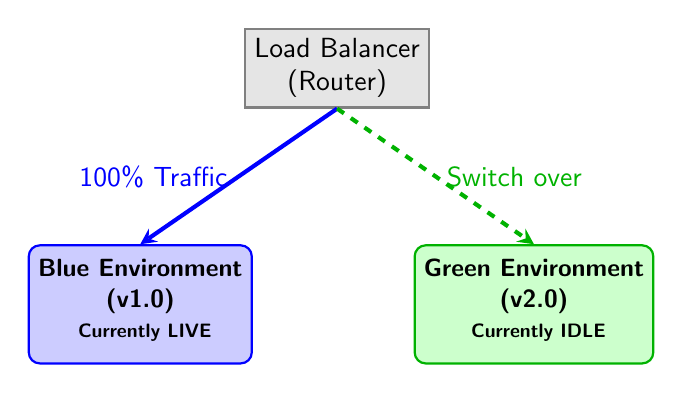
\begin{tikzpicture}[
        server/.style={rectangle, thick, minimum width=2.5cm, minimum height=1.5cm, align=center, font=\small\bfseries, rounded corners},
        router/.style={rectangle, draw=gray, fill=gray!20, thick, minimum width=2cm, minimum height=1cm, align=center},
        arrow/.style={->, >=stealth, line width=1.5pt}
    ]
        % Nodes
        \node[router] (loadbalancer) at (0, 3) {Load Balancer\\(Router)};
        \node[server, draw=blue, fill=blue!20] (blue) at (-2.5, 0) {Blue Environment\\(v1.0)\\ \vspace{0.1cm} \scriptsize Currently LIVE};
        \node[server, draw=green!70!black, fill=green!20] (green) at (2.5, 0) {Green Environment\\(v2.0)\\ \vspace{0.1cm} \scriptsize Currently IDLE};
        
        % Traffic arrow (Active)
        \draw[arrow, blue] (loadbalancer.south) -- (blue.north) node[midway, left, text=blue] {100\% Traffic};
        
        % Switch arrow (Dashed)
        \draw[arrow, green!70!black, dashed] (loadbalancer.south) -- (green.north) node[midway, right, text=green!70!black] {Switch over};
    \end{tikzpicture}
    
    \vspace{0.2cm}
    \small
    \begin{itemize}
        \item Spin up an exact clone of your production environment (Green).
        \item Deploy V2 to Green. Run tests on it \textit{while it is invisible to users}.
        \item When ready, flip the Load Balancer router. Blue becomes idle, Green becomes live. Zero downtime. Instant rollback if things break.
    \end{itemize}
\end{frame}

\begin{frame}
    \frametitle{Canary Releases}
    Named after the ``Canary in a Coal Mine''.

    \centering
    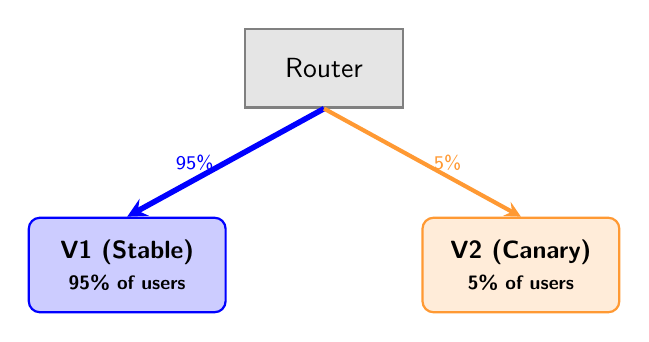
\begin{tikzpicture}[
        server/.style={rectangle, thick, minimum width=2.5cm, minimum height=1.2cm, align=center, font=\small\bfseries, rounded corners},
        router/.style={rectangle, draw=gray, fill=gray!20, thick, minimum width=2cm, minimum height=1cm, align=center},
        arrow/.style={->, >=stealth, line width=1.5pt}
    ]
        \node[router] (lb) at (0, 2.5) {Router};
        \node[server, draw=blue, fill=blue!20] (v1) at (-2.5, 0) {V1 (Stable)\\\scriptsize 95\% of users};
        \node[server, draw=orange!80, fill=orange!15] (v2) at (2.5, 0) {V2 (Canary)\\\scriptsize 5\% of users};
        \draw[arrow, blue, line width=2pt] (lb.south) -- (v1.north) node[midway, left, font=\scriptsize, text=blue] {95\%};
        \draw[arrow, orange!80] (lb.south) -- (v2.north) node[midway, right, font=\scriptsize, text=orange!80] {5\%};
    \end{tikzpicture}

    \vspace{0.1cm}
    \begin{itemize}
        \item Monitor V2 error logs for 1 hour. No crashes? Dial up to 20\%, 50\%, 100\%.
        \item \textbf{Benefit:} A catastrophic bug in V2 only affects \textbf{5\%} of users, not 100\%.
    \end{itemize}
\end{frame}

\begin{frame}
    \frametitle{Canary vs. Blue/Green: When to Use Each?}
    \small
    \begin{center}
    \begin{tabular}{p{3.5cm} p{3cm} p{3cm}}
        \hline
        \rowcolor{gray!30}
        \textbf{Situation} & \textbf{Blue/Green} & \textbf{Canary} \\
        \hline
        \rowcolor{gray!15}
        Database schema changes & \textcolor{green!60!black}{\textbf{Often preferred}} & \textcolor{red}{\textbf{Higher risk}} \\
        Gradual confidence building & Harder & \textcolor{green!60!black}{\textbf{Well-suited}} \\
        \rowcolor{gray!15}
        Instant rollback needed & \textcolor{green!60!black}{\textbf{Fast (single switch)}} & Slower (dial back) \\
        Infrastructure cost & Higher (2 envs) & Lower \\
        \rowcolor{gray!15}
        User-facing A/B testing & Less common & \textcolor{green!60!black}{\textbf{Common}} \\
        \hline
    \end{tabular}
    \end{center}

    % \vspace{0.3cm}
    % \begin{block}{Discussion (2 min)}
    %     Your GCS needs to deploy a breaking database schema change tonight. Which strategy do you choose, and why? What extra steps would you need?
    % \end{block}
\end{frame}

\begin{frame}
    \frametitle{Knowledge Check: Choose the Strategy}
    \textbf{Scenario:} You are deploying an update to the Ground Control Station that fundamentally alters the database schema (changing how coordinates are stored). 
    
    \vspace{0.2cm}
    \textbf{Question:} In a shared-database setup, which deployment strategy is typically the \textit{highest risk} to use here?
    \begin{enumerate}
        \item A) Blue/Green Deployment
        \item B) Canary Release
        \item C) Big Bang Deployment
    \end{enumerate}
    
    \pause
    \vspace{0.2cm}
    \begin{alertblock}{Answer: B (Canary Release)}
        Canary releases run V1 and V2 \textbf{simultaneously}. If V2 writes new schema data to the database, V1 will crash because it doesn't understand the new format! Database-breaking changes usually require Blue/Green (with careful DB replication) or a brief Big Bang maintenance window.
    \end{alertblock}
\end{frame}

%------------------------------------------------------------
\section{Release Control with Feature Flags}
%------------------------------------------------------------

\begin{frame}
    \frametitle{Deployment $\neq$ Release}
    One of the most powerful concepts in modern DevOps is decoupling the act of \textit{deploying} code from the act of \textit{releasing} a feature.
    
    \begin{itemize}
        \item \textbf{Deploying:} Putting the code on the production server.
        \item \textbf{Releasing:} Making that code visible/active for the end user.
    \end{itemize}
    
    \vspace{0.3cm}
    How do we push a half-finished feature to production servers without breaking the application for users? \textbf{Feature Flags (Toggles).}
\end{frame}

\begin{frame}[fragile]
    \frametitle{Implementing Feature Flags}
    Feature flags are often implemented as conditionals around new code paths, controlled by external configuration (for example env vars, config files, or a flag service).
    
    \begin{minted}[bgcolor=lightgray, fontsize=\tiny]{python}
import os

# Read the flag from environment variables (defaults to False)
ENABLE_NEW_DASHBOARD = os.getenv("FF_NEW_DASHBOARD", "false").lower() == "true"

@app.get("/api/dashboard")
def get_dashboard_data():
    if ENABLE_NEW_DASHBOARD:
        # The new V2 code you are currently working on
        return fetch_advanced_telemetry()
    else:
        # The old, stable V1 code that users currently see
        return fetch_basic_telemetry()
    \end{minted}

    \vspace{0.2cm}
    \textbf{The Power:} Deploy this to production many times a day. When ready to launch, change the environment variable to \texttt{"true"}. \textbf{No redeployment needed!}
\end{frame}

% NEW SLIDE: Feature Flag Pitfalls — connecting back to Week 12
\begin{frame}
    \frametitle{Feature Flag Pitfalls: Flag Debt}
    \small
    Feature flags are powerful, but they come with a hidden cost you should recognise from last week.

    % \vspace{0.2cm}
    % \begin{alertblock}{Flag Debt — a form of Technical Debt (Week 12)}
    %     Every flag is an \texttt{if} branch that \textbf{must be maintained forever} until it is removed. A codebase with 50 forgotten flags becomes impossible to reason about.
    % \end{alertblock}

    \vspace{0.2cm}
    \textbf{Common pitfalls:}
    \begin{itemize}
        \item \textbf{Flags that never get cleaned up} — the old code path stays in the repo indefinitely, adding complexity (Lehman's 2nd Law!).
        \item \textbf{Testing explosion} — with $n$ flags, you theoretically have $2^n$ code paths to test.
        \item \textbf{Flag coupling} — flags that depend on other flags create hidden interactions and bugs.
    \end{itemize}

    \vspace{0.1cm}
    \begin{block}{Rule of Thumb}
        When a flag is fully rolled out, \textbf{schedule its removal} in the same sprint. Treat it like any other item in your Technical Debt Register.
    \end{block}
\end{frame}

\begin{frame}
    \frametitle{How They Combine in Practice}
    \small
    Deployment mechanics and feature flags are strongest when used together.

    \vspace{0.2cm}
    \begin{itemize}
        \item \textbf{Canary + Flags:} Send 5\% traffic to V2, but keep risky features off by default. Enable per cohort as confidence grows.
        \item \textbf{Blue/Green + Flags:} Switch infrastructure instantly, then progressively enable new features without redeploying.
        \item \textbf{Dark Launch + Flags:} Deploy code to production, keep UI hidden, and validate behavior/metrics before public release.
    \end{itemize}

    \vspace{0.2cm}
    \begin{block}{Operational Safety Net}
        Keep a \textbf{kill switch} flag for high-risk functionality so you can disable exposure quickly while investigating incidents.
    \end{block}
\end{frame}

%------------------------------------------------------------
\section{Next Steps}
%------------------------------------------------------------

% NEW SLIDE: Lecture summary tying everything together
\begin{frame}
    \frametitle{Lecture Summary: The Full Picture}
    \centering
    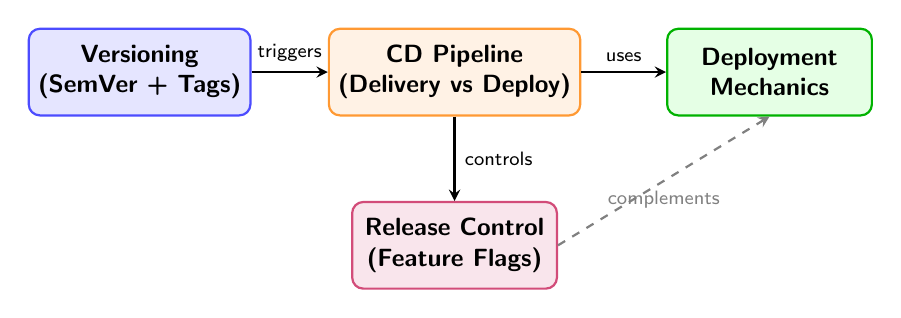
\begin{tikzpicture}[
        box/.style={rectangle, rounded corners, thick, minimum width=2.6cm, minimum height=1.1cm, align=center, font=\small\bfseries},
        arrow/.style={->, >=stealth, thick}
    ]
        \node[box, draw=blue!70, fill=blue!10]   (ver)   at (0, 0)    {Versioning\\(SemVer + Tags)};
        \node[box, draw=orange!80, fill=orange!10] (cd)  at (4, 0)    {CD Pipeline\\(Delivery vs Deploy)};
        \node[box, draw=green!70!black, fill=green!10] (strat) at (8, 0) {Deployment\\Mechanics};
        \node[box, draw=purple!70, fill=purple!10] (ff)  at (4, -2.2) {Release Control\\(Feature Flags)};

        \draw[arrow] (ver) -- (cd) node[midway, above, font=\scriptsize] {triggers};
        \draw[arrow] (cd) -- (strat) node[midway, above, font=\scriptsize] {uses};
        \draw[arrow] (cd.south) -- (ff.north) node[midway, right, font=\scriptsize] {controls};
        \draw[arrow, dashed, gray] (ff.east) -- (strat.south) node[midway, below, font=\scriptsize, text=gray] {complements};
    \end{tikzpicture}

    \vspace{0.3cm}
    \small Together these practices make deployments \textbf{traceable, safe, and invisible to end-users} — the goal from slide 5.
\end{frame}

\begin{frame}
    \frametitle{This Week's Lab: Release Management}
    In the workshop, you will practice managing releases for your Ground Control Station.
    
    \begin{itemize}
        \item \textbf{Task 1: Semantic Versioning:} Determine the correct SemVer numbers for various scenarios in your project.
        \item \textbf{Task 2: Git Tagging \& GitHub Releases:} Create formal annotated tags and generate a changelog using GitHub Releases.
        \item \textbf{Task 3: Feature Flags:} Implement an environment-variable-driven Feature Flag in your backend API to hide a newly developed feature.
    \end{itemize}
\end{frame}

% \begin{frame}
%     \frametitle{Reading \& Resources}
%     \begin{itemize}
%         \item \textbf{Semantic Versioning Specs:} \url{https://semver.org/} --- \textit{The official 11-point rulebook for SemVer.}
%         % \item \textbf{Martin Fowler on Feature Toggles:} \url{https://martinfowler.com/articles/FeatureToggles.html}
%         \item \textbf{GitHub Documentation:} \textit{Managing Releases in a Repository.}
%     \end{itemize}
% \end{frame}

% EXPANDED next-lecture slide
\begin{frame}
    \frametitle{Next Lecture}
    
    
    \begin{center}
        \textbf{LEPSI, Security \& Professional Practice}
    \end{center}
\end{frame}

\begin{frame}
    \frametitle{Q \& A}
    \begin{center}
        \Huge Any Questions?\\\vspace{0.5cm} 
        \normalsize fdelduchetto@lincoln.ac.uk
    \end{center}
\end{frame}

\end{document}